%%%%%%%%%%%%%%%%%%%%%%%%%%%%%%%%%%%%%%%%%%%%%%%%%%%%%%%%%%%%%%%%%%%%%%%%%%%%%%%%
%2345678901234567890123456789012345678901234567890123456789012345678901234567890
%        1         2         3         4         5         6         7         8

%\documentclass[letterpaper, 10 pt, conference]{ieeeconf}  % Comment this line out
                                                          % if you need a4paper
\documentclass[a4paper, 10pt, conference]{ieeeconf}      % Use this line for a4
                                                          % paper

\IEEEoverridecommandlockouts                              % This command is only
                                                          % needed if you want to
                                                          % use the \thanks command
\overrideIEEEmargins
% See the \addtolength command later in the file to balance the column lengths
% on the last page of the document

\usepackage{graphicx} %package to manage images
\graphicspath{ {./images/} }
\usepackage{wrapfig}

% The following packages can be found on http:\\www.ctan.org
\usepackage{graphics} % for pdf, bitmapped graphics files
\usepackage{epsfig} % for postscript graphics files
\usepackage{mathptmx} % assumes new font selection scheme installed
\usepackage{times} % assumes new font selection scheme installed
\usepackage{amsmath} % assumes amsmath package installed
\usepackage{amssymb}  % assumes amsmath package installed
\usepackage{array}

\newcommand{\squeezeup}{\vspace{-2.5mm}}

\title{\LARGE \bf
Did the Google+ User Network Foreshadow It’s Demise?
}

\author{
\textbf{Adnan Salehin}\\
\textit{a.salehin@se16.qmul.ac.uk}\\
\small Writing Python Programs\\
\small with NetworkX,\\
\small Matplotlib and Numpy.\\
\small Producing sub-graphs and\\ 
\small applying algorithms.\\
\small Data analysis on chosen metrics\\ 
\small and producing charts.\\
\small Report writing for relevant sections.\\
\textbf{Percentage: 35{\%}} \and 
\textbf{Laraib Azam Rajper}\\
\textit{l.azam@se15.qmul.ac.uk}\\
\small Research and applications\\
\small of relevant papers.\\
\small Analysis of Paper 1 and 2\\ 
\small in Related Works,\\
\small Dataset {\&} Statistics\\
\small and Terminology sections\\
\small and drawing of conclusions.\\
\small Referencing and citation.\\
\textbf{Percentage: 33{\%}} \and 
\textbf{Elif Sebnem Cudi}\\ 
\textit{e.s.cudi@se15.qmul.ac.uk}\\
\small Gephi Illustrations\\
\small Abstract, Introduction and\\
\small problem definition write up\\
\small LaTeX write up.\\
\small Referencing and citation.\\
\textbf{Percentage: 32{\%}}}

% % \author{Huibert Kwakernaak$^{1}$ and Pradeep Misra$^{2}$% <-this % stops a space
% % \thanks{*This work was not supported by any organization}% <-this % stops a space
% % \thanks{$^{1}$H. Kwakernaak is with Faculty of Electrical Engineering, Mathematics and Computer Science,
% %         University of Twente, 7500 AE Enschede, The Netherlands
% %         {\tt\small h.kwakernaak at papercept.net}}%
% % \thanks{$^{2}$P. Misra is with the Department of Electrical Engineering, Wright State University,
% %         Dayton, OH 45435, USA
% %         {\tt\small p.misra at ieee.org}}%
% }


\begin{document}
\maketitle            
\thispagestyle{plain}
\pagestyle{plain}

%%%%%%%%%%%%%%%%%%%%%%%%%%%%%%%%%%%%%%%%%%%%%%%%%%%%%%%%%%%%%%%%%%%%%%%%%%%%%%%%
\begin{abstract}

Google will be shutting down Google+ for its consumers on April 2nd, 2019. This is the result of poor understanding of user requirements and lack of a unique selling point. This study will explore the ways in which the user network of Google+ can reflect its low user engagement when compared with a rival social networking platform of similar scale. Sample networks from Google+ and Twitter are used to calculate their degree assortativity and reciprocity. The findings show that Twitter has a more cohesive network with users that are more likely to reciprocate a connection, while Google+ users are less likely to form subgroups that are highly connected.

\end{abstract}

%%%%%%%%%%%%%%%%%%%%%%%%%%%%%%%%%%%%%%%%%%%%%%%%%%%%%%%%%%%%%%%%%%%%%%%%%%%%%%%%
\section{INTRODUCTION}

\textit{"90 percent of Google+ user sessions are less than five seconds."}\cite{c1}. This is a quote from the blog post released by Google on October 18th, 2018, where they announced that they will be terminating their Google+ service for their consumers. The news came after a massive data breach that affected around 500,000 users. In the same post, it was admitted that both consumer and developer adoption was lower than expected.

Throughout Google+'s lifetime, Google invested heavily into the marketing of their online social network (OSN), with events such as Google+ hangout calls with ISS astronauts, as well as the former US President Barack Obama \cite{c2} in order to attract more users. However, even the popularity of these events were made possible by the use of Twitter and Facebook tools, which indicated a fundamental problem with the premise of Google+. Google have also enlarged their user base with not-so-ethical means, such as forcing all YouTube users who want to use 
the commenting feature of the website to create Google+ accounts \cite{c3}. Experiments conducted by the likes of Digital Doughnut \cite{c4} and SEO-Hacker \cite{c5} also reveal that creating a Google+ business page can be used for search engine optimisation (SEO) as Google can integrate the social signals generated by Google+ higher in their search engine rankings than those generated by their competitors.

\subsection{Problem Statement}
As of 2016, 91 percent of all Google+ accounts are empty \cite{c6}. Robert Hof of Forbes explains that Google cannot define what Google+ is meant to be to its users, as there are no unique features that sets it apart from its competitors \cite{c7}. This can be seen as the theoretical reason for its low user activity, but we want to prove Google+'s failure using the power of networks.

Our hypothesis is that, with so many empty accounts, users should not have a high amount of following or follower connections. For those who do, they are likely to be accounts that are not related to each other in real life context. This means that there will be less communities in a Google+ network as supposed to a social networking site that has high user engagement. 

\section{RELATED WORK}

\subsection{Tracing the Birth of an OSN: Social Graph and Profile Analysis in Google+ \cite{c13}}

June 2011 saw the launch of Google+, which has been Google's largest endeavor into the OSN market to date. The Google+ OSN differed to other major players like Facebook and Twitter due to the fact that it was backed by a company which monopolises the data industry, therefore providing the unique opportunity to offer much more than just an OSN. Schi\"oberg et al \cite{c13} provides an insightful analysis on the growth and downfall of the Google+ OSN, where the research was based on 16 crawls of the Google+ social graph or the user profiles, analysed over a 2 month period which included 40 million users. Securitising the data helped identify user behaviours, social dependencies, dynamics and changes over time. Identification of such factors is crucial as it provides a precedent for other social networks which either exist or are industry incumbents. Through utilising the findings they can improve either own products and avoid the mistakes made which lead to the downfall of Google+. Schi\"oberg et al \cite{c13} present in their findings as follows:
\linebreak
\subsubsection{In/Out Degree}
When observing the structure of the Google+ network, it can be observed by its In/Out Degree figures that the network can not be classified as perfectly asymmetrical as Twitter can. However, the network also does not display characteristics of symmetrical networks like Flickr, meaning that it is unique in its features and within the OSN ecosystem.

During the initial release of the network and its significant growth in the time that followed there was a decrease in its mean and median out degree. Further analysis by Schi\"oberg et al \cite{c13} identified that this was due to an increase in the number on “lonely” nodes and weakly connected components in the networks social graph when compared to the period directly after its launch.
\linebreak
\subsubsection{User Profiles}

Characteristics of the user profiles indicate that the Google+ OSN is used predominantly by a professional audience of university students or IT professionals and that while 50 percent of used operate within the same time zone, the majority and separated by distances exceeding 1000km. Thus, user distances typical spam over larger geographical areas when compared with Twitter. 

The total probability that information is shared by users within the network is only at 25 percent or less, drastically lower then Twitter. Overall, indicating to the low usage of the network when compared with Twitter who supports a more engaged global audience of various professions.

\subsection{Robustness of Social Networks: Comparative Results Based on Distance Distributions \cite{c15}}

Boldi et al \cite{c15} conducted an investigation on the robustness of social networks, more specifically they worked to identify the highest impact that would be made when a given node within a network was removed. Their paper aims to determine the centrality of a given node in a given network and the effects of its centrality on the network as a whole. This applies to our investigation as it allows us to identify the importance that a node within our social networks has on its communities and how central it is to the the interaction of the users around it. In the case of Google+, would the network have better user engagement and thus a higher correlation coefficient?

However, Boldi et al \cite{c15} go on to explain in their findings that social networks are extremely resistant to node removal, thus there can be no guarantee that removal on the “lonely” nodes as suggested by Schi\"oberg et al \cite{c13} would strengthen the Google+ network, decreasing its shortest path and acting as a boost for user engagement.

Boldi et al \cite{c15} suggest that the strength of a social network can be determined through its strongest nodes which can be located at the center of its communities or "hubs". The hubs of a network in our case would be those users who act as bridges between clusters, fostering relationships and networking across various communities. Thus, indicating that a feature of successful networks would be a high clustering coefficient, high reciprocity levels and a high number of bridges, all of which can be identified within the Twitter network.

\section{DATA SETS}

The two data sets being used are from Stanford University. Both represent directed networks with the nodes representing users, and edges representing the act of one user following another user in Twitter's case, and a user being in another user's circle in the case of Google+. The initial Google+ \cite{c11} data contained over 100,000 nodes and 10 million edges, while the Twitter \cite{c10} data contained over 80,000 nodes and 1 million edges. Networks of this size were not computationally feasible to visualize and perform analysis on since many of our metrics implement algorithms of $O(n^2)$ and above. Therefore, 3 samples were taken from both data sets, each consisting of 1000 nodes. The 6 samples were compared by taking the mean of the 3 samples of each of the Google+ and Twitter networks. The Google+ and Twitter data sets were represented by orange and blue colours respectively in our poster. In addition, below we have identified our in-depth statistical analysis, which utilises figures generated using NetworkX.

\subsection{Terminology}

\begin{itemize}
\item \textbf{Nodes:} Each user within the Google+ and Twitter social graphs is represented by a node/vertices. 
\item \textbf{Edges:} Given that the Edge between A and B is directed. A $\rightarrow$ B represents that user A included user B in one of his circles. In the instances that  user B has also included user A in his circles the graph contains another directed edge B $\rightarrow$ A.
\item \textbf{Modularity:} This measure identifies that strength of divisions within a network into modules or clusters/communities.
\item \textbf{Communities:} This measure identifies the number of divisions within a network into clusters or modules.
\item \textbf{Diameter:} This measure identifies that shortest distance travel between the two most distance nodes within a network. 
\item \textbf{Average Path Length:} This measure identifies the number of edges contained within an average path from one node to another.
\item \textbf{Out Degree:} The Out Degree identifies the number of directed Edges that begin at a specific node.
\item \textbf{In Degree:} The In Degree identifies the number of directed Edges that conclude at a specific node.
\item \textbf{Clustering Coefficient:} This measure indicates the degree to which member or nodes within a network tend to cluster together.
\end{itemize}

\begin{table}[htb]
\caption{Google+ Statistics}
\label{table_google}
\begin{center}
\begin{tabular}{ | l | l | } 
\hline
\textbf{Statistic} & \textbf{Mean Value of 3 Samples (4 s.f.)}\\
\hline
Nodes & 1000\\
Edges & 4762\\
Modularity & 0.4123\\
Number of Communities & 77.0\\
Diameter & 10.33\\
Average Path Length & 3.283\\
Average (In/Out) Degree & 47.62\\
Average Clustering Coefficient & 0.3160\\
Reciprocity & 0.4342\\
Assortativity & -0.0632\\
\hline
\end{tabular}
\end{center}
\end{table}

\begin{table}[htb]
\caption{Twitter Statistics}
\label{table_twitter}
\begin{center}
\begin{tabular}{ | l | l | } 
\hline
\textbf{Statistic} & \textbf{Mean Value of 3 Samples (4 s.f.)}\\
\hline
Nodes & 1000\\
Edges & 1724\\
Modularity & 0.7387\\
Number of Communities & 28.67\\
Diameter & 13.00\\
Average Path Length & 4.496\\
Average (In/Out) Degree & 17.24\\
Average Clustering Coefficient & 0.4042\\
Reciprocity & 0.5744\\
Assortativity & 0.0873\\
\hline
\end{tabular}
\end{center}
\end{table}

\section{APPROACH}
The goal of this paper was to establish a set of metrics to clearly identify which of the two networks exhibit more “cohesion” between the nodes. The study was to observe if there is any clear indication that one of the networks is performing better or worse in this regard. In order to do a fair comparison of such large networks, 3 samples of sub-graphs of each network were extracted from our available edgelist data where each sub-graph consisted of 1000 nodes. The total of 6 samples were tested with two different algorithms, and the results and their averages were compared.

For the first algorithm, the evaluation of the \textbf{degree assortativity coefficient} value was chosen. This is the product moment correlation coefficient (also known as Pearson correlation coefficient) between similar degrees in the network. The algorithm used for the purpose of this paper also takes into account other factors such as standard deviation values. Typically, for a well connected social network we expect that it will consist of several smaller clusters of communities. This would result in a positive degree assortativity value which is perhaps less than 0.5 (a value of 1 represents 100 percent correlation, whereas 0 represents 0 percent correlation) since we are expecting some connections between nodes of similar degrees. 

In other words, for a well connected network, we expect to see some people to connect with other people with similar number of friends/followers. The other case is a negative assortativity value, which would imply that there is a tendency in the network to form abnormally large clusters with a lower total number of clusters. This would result in the network appearing to be somewhat disassortative because the tendency would be to focus on certain central nodes.
This was calculated using the NetworkX Python library. The function implements the following equation:

\[
r = \frac{\sum_{xy}xy(e_{xy}-a_xb_y)}{\sigma_a\sigma_b}
\]

Where $a_x$ and $b_y$ are, respectively, the fraction of edges that start and end at nodes with values $x$ and $y$ and, $\sigma_a$ and $\sigma_b$ are the standard deviations of the distributions $a_x$ and $b_y$. The value of $r$ lies in the range $−1 \leq r \leq 1$, with $r = 1$ indicating perfect assortativity and $r = −1$ indicating perfect disassortativity \cite{c12}.

The second algorithm that was chosen was \textbf{reciprocity}. Reciprocity is the measure of the number of nodes in a directed graph that reciprocate a connection, i.e. the connection is reciprocal if it goes both ways. In this case the Garlaschelli and Loffredo definition of reciprocity \cite{c9} is being used. This is defined as the correlation coefficient between the entries of the adjacency matrix of a directed graph. The adjacency matrix denotes whether pairs of nodes in the graph are adjacent (i.e. linked). The reciprocity defined as such is given by:

\[
\rho \equiv \frac{\sum_{i\neq j}(a_{ij}-\bar{a})(a_{ji}-\bar{a})}{\sum_{i\neq j}(a_{ij}-\bar{a})^2}
\]
Where the average value $\bar{a}$ is given by:
\[
\bar{a} \equiv \frac{\sum_{i\neq j} a_{ij}}{N(N-1)} = \frac{L}{N(N-1)}
\]
Here $\rho$ represents the reciprocity, $L$ represents the total number of links between nodes, $N$ represents the total number of nodes, $a_{ij} = 1$ if a link from $i$ to $j$ is there, and $a_{ij} = 0$ if not.

Both of the networks that were analysed were in the form of directed graphs. Thus, it would be a fair comparison to calculate how many of the nodes actually reciprocate a connection. Reciprocity is often overlooked as a minor measure in graphs, but in this case, it is a vital measure. For Google+, a reciprocal connection implies both users have each other in their respective “circle” and for Twitter it implies that both users follow each other. 
For a well connected network we are expecting to see a higher value for the ratio of reciprocal connections to the total number of connections (reciprocity value).

\section{RESULTS}

\subsection{Analysis of Degree Assortativity}

\begin{table}[htb]
\caption{Degree Assortativity Results}
\begin{center}
\begin{tabular}{ | l | l | l |} 
\hline
& \textbf{Google+} & \textbf{Twitter}\\[0.5ex]
\hline
Sample 1 & -0.1417 & +0.1963\\
Sample 2 & -0.06215 & -0.0362\\
Sample 3 & +0.0141 & +0.1017\\[0.5ex]
\hline
\textbf{Average Value} & \textbf{-0.0632} & \textbf{+0.0873}\\[0.5ex]
\hline
\end{tabular}
\end{center}
\end{table}

The average assortativity values in Table III indicate that Twitter has a more cohesive network as in this network, nodes with similar degrees are more likely to be connected than the Google+ network. The Google+ network has a slight positive correlation between nodes with dissimilar degrees. The Twitter network on the other hand has a positive correlation between nodes with similar degrees. Moreover, from the magnitude of these values alone, it can be concluded that the Twitter network is more assortative than Google+ (which is more disassortative).

In addition to this calculation, the average neighbour degree values was plotted against degree values using the NetworkX and Matplotlib libraries in Python averaging over 3 samples for each network. This was done to observe the correlation between similar degrees for the two networks and have a better grasp of the degree assortativity of these networks.

\begin{figure}[thpb]
      \centering
      \framebox{\parbox{3in}{
      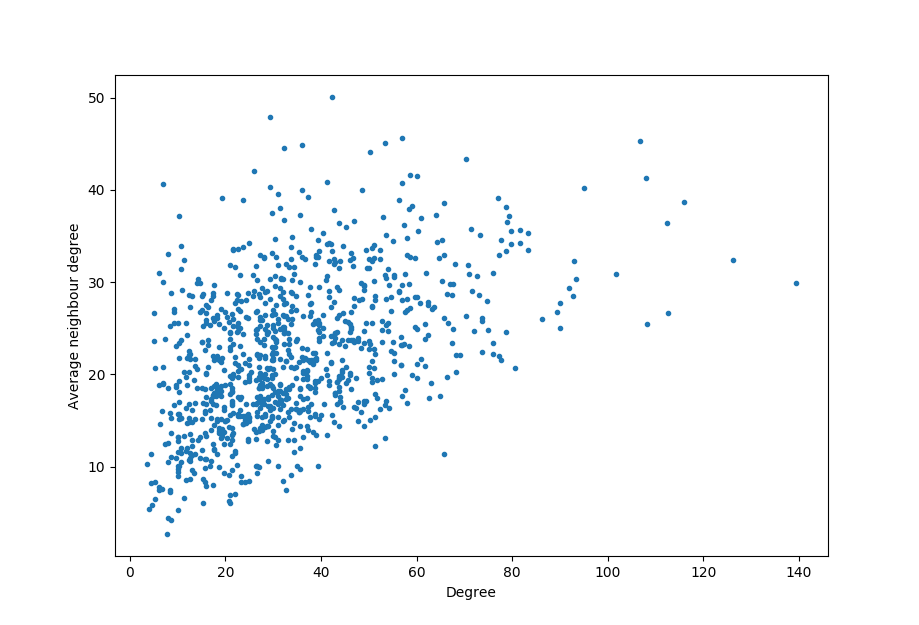
\includegraphics[width=0.45\textwidth]{image3.png}}}
      \caption{Degree assortativity plot for Twitter}
      \label{figurelabel}
   \end{figure}
   
\begin{figure}[thpb]
      \centering
      \framebox{\parbox{3in}{
      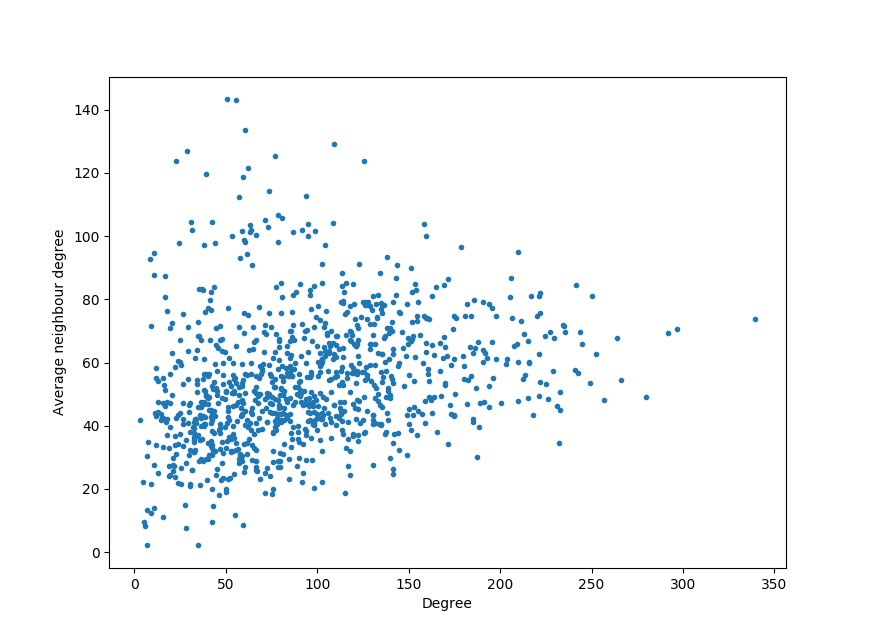
\includegraphics[width=0.45\textwidth]{image4.png}}}
      \caption{Degree assortativity plot for Google+}
      \label{figurelabel}
   \end{figure}
   
Furthermore, the \textbf{Pearson Correlation Coefficient} was calculated for the graphs shown in Fig. 1 and Fig. 2. This was done using the NumPy Python library. Google+ had a value of +0.2564 and Twitter had a value of +0.4619. This further demonstrates that the Twitter network has a higher tendency to have edges between nodes of similar degrees.

\subsection{Analysis of Garlaschelli and Loffredo Reciprocity}

\begin{table}[htb]
\caption{Reciprocity Results}
\begin{center}
\begin{tabular}{ | l | l | l |} 
\hline
& \textbf{Google+} & \textbf{Twitter}\\[0.5ex]
\hline
Sample 1 & 0.2835 & 0.5669\\
Sample 2 & 0.5882 & 0.5376\\
Sample 3 & 0.4308 & 0.6188\\[0.5ex]
\hline
\textbf{Average Value} & \textbf{0.4342} & \textbf{0.5744}\\[0.5ex]
\hline
\end{tabular}
\end{center}
\end{table}

The average reciprocity values in Table IV clearly shows that the Twitter network has nodes which are more likely to reciprocate a connection, i.e. a randomly selected Twitter user is more likely to follow a follower back when compared to Google+ where users are less likely to have someone in their circle even if they are in the other user’s circle.

\subsection{Further Statistics that Support Our Hypothesis}

Based on the analysis above, it can hypothesized that the Google+ network is performing poorly when compared to the Twitter network on our chosen metrics. To draw more conclusions regarding the hypothesis, other standard properties of networks will be compared. For all calculations, 3 sub-graphs of 1000 nodes each were taken from the primary data set for each network. The average value of each data point has been used to produce the results and the corresponding graphs.

\begin{figure}[thpb]
      \centering
      \framebox{\parbox{3in}{
      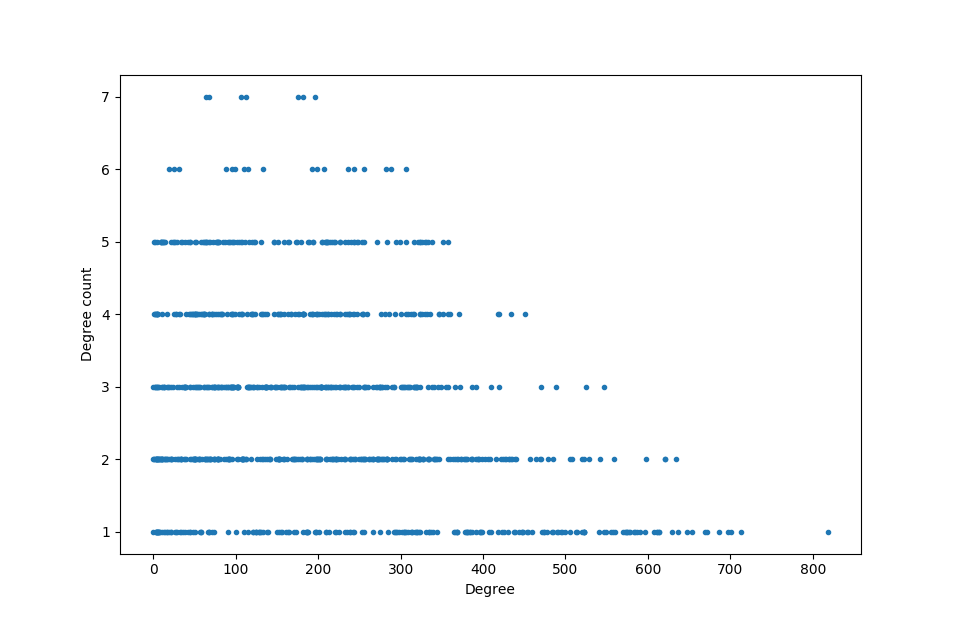
\includegraphics[width=0.45\textwidth]{image15.png}}}
      \caption{Degree distribution plot for Google+}
      \label{figurelabel}
   \end{figure}

\begin{figure}[thpb]
      \centering
      \framebox{\parbox{3in}{
      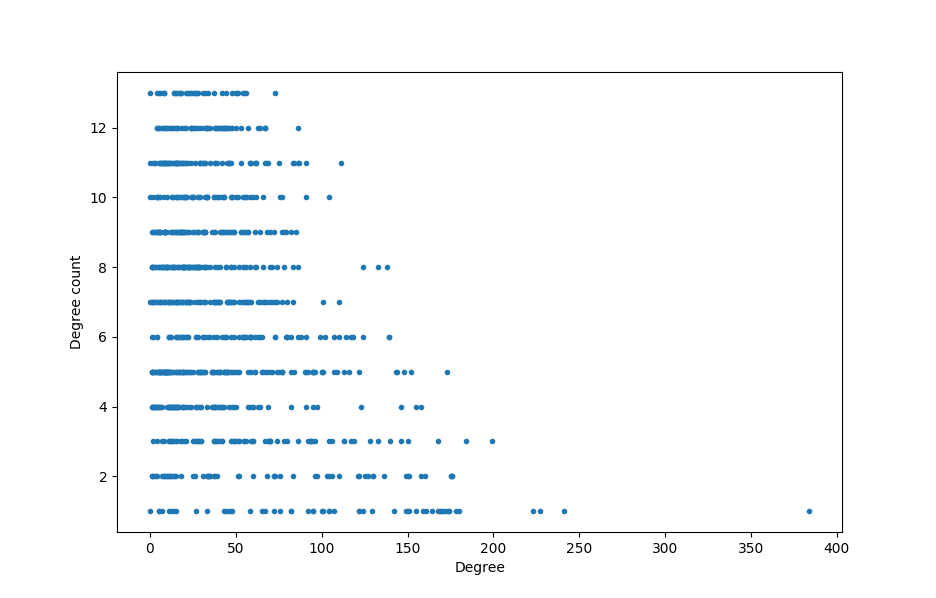
\includegraphics[width=0.45\textwidth]{image13.png}}}
      \caption{Degree distribution plot for Twitter}
      \label{figurelabel}
   \end{figure}
   
\subsubsection{Degree Distribution}
Analyzing the degree distributions for Google+ and Twitter in Figure 3 and 4 respectively, it can be seen that with an increase in degree value, the count generally decreases for both graphs. It can be see that the number of nodes with degree values over 400 in the Google+ network is in the range of 1 to 4, which is an advantage over the Twitter network since the maximum degree it exhibits is around 380. However, even for a degree value of 100 for example, the Twitter network has almost twice the count value compared to Google+. It can be argued that this overtakes the previously mentioned advantage of the Google+ network as it shows that Twitter has many cases with more nodes at the same degree value.

\begin{figure}[thpb]
      \centering
      \framebox{\parbox{3in}{
      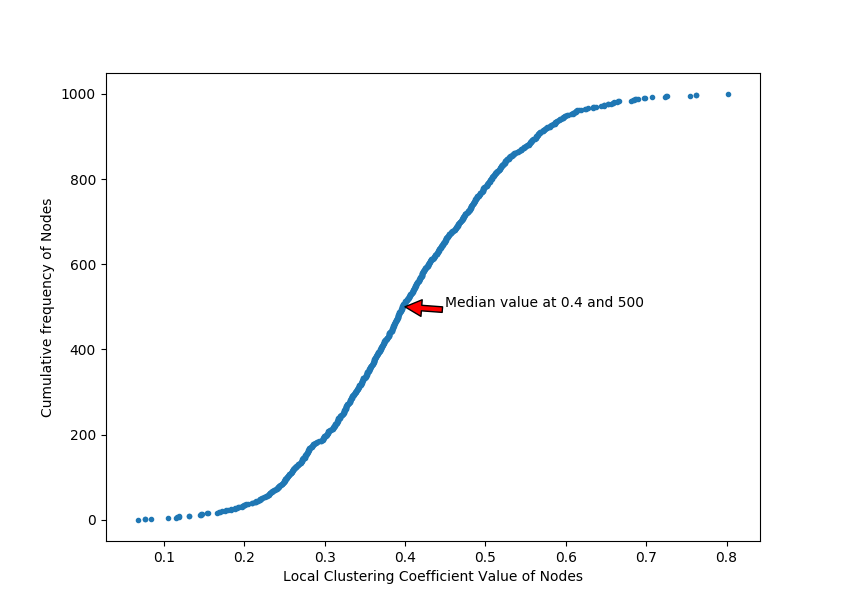
\includegraphics[width=0.45\textwidth]{image1.png}}}
      \caption{Cumulative frequency graph for local clustering coefficient (Twitter)}
      \label{figurelabel}
   \end{figure}
   
\begin{figure}[thpb]
      \centering
      \framebox{\parbox{3in}{
      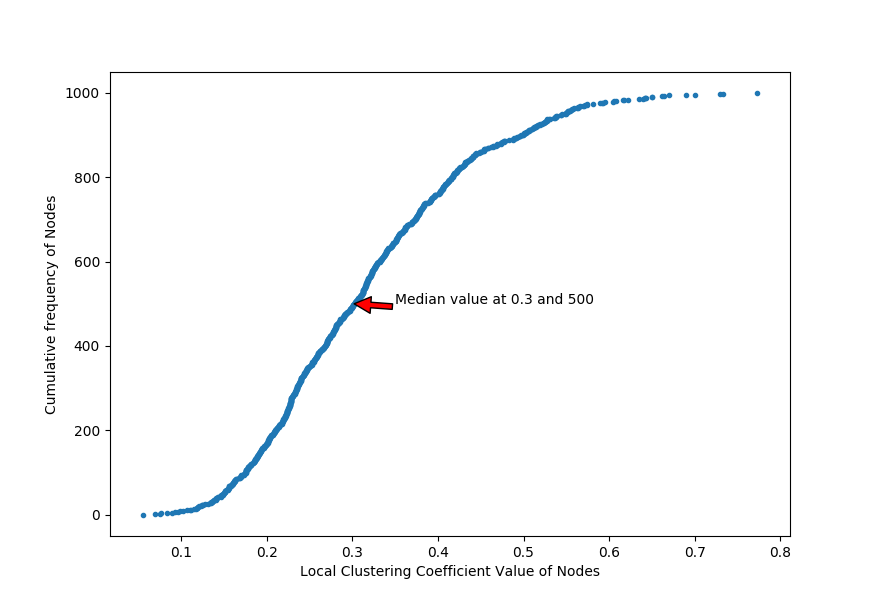
\includegraphics[width=0.45\textwidth]{image6.png}}}
      \caption{Cumulative frequency graph for local clustering coefficient (Google+)}
      \label{figurelabel}
   \end{figure}

\subsubsection{Clustering coefficient}
From the cumulative frequency distributions of the clustering coefficients of the two networks in Figure 5 and Figure 6, it is seen that the Twitter network has a higher median value of 0.4 and the Google+ network has a median of 0.3. A higher value here indicates a more cohesive network. The trend is apparent in the general shapes of the graphs as well. This implies that Twitter users are more likely to form subgroups or clusters that are highly connected, than Google+ users.
The local clustering coefficient for a vertex is given by the proportion of links between the vertices within its neighbourhood divided by the number of links that could possibly exist between them. 
Thus, the \textbf{local clustering coefficient for directed graphs} is given as \cite{c14}:

\[
C_i = \frac{|\{e_{jk}:v_j,v_k \in N_i,e_{jk} \in E\}|}{k_i(k_i-1)}
\]

\begin{figure}[thpb]
      \centering
      \framebox{\parbox{3in}{
      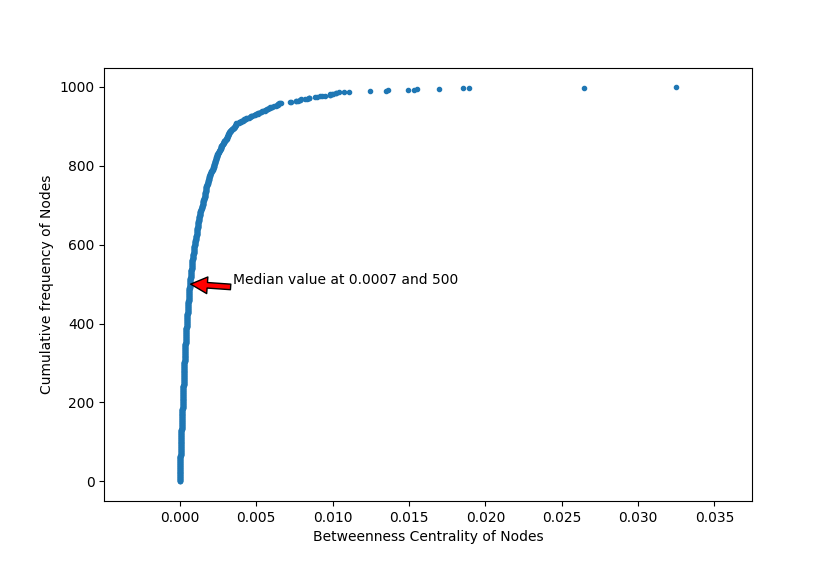
\includegraphics[width=0.45\textwidth]{image8.png}}}
      \caption{Cumulative frequency graph for betweenness centrality (Google+)}
      \label{figurelabel}
   \end{figure}
   
\begin{figure}[thpb]
      \centering
      \framebox{\parbox{3in}{
      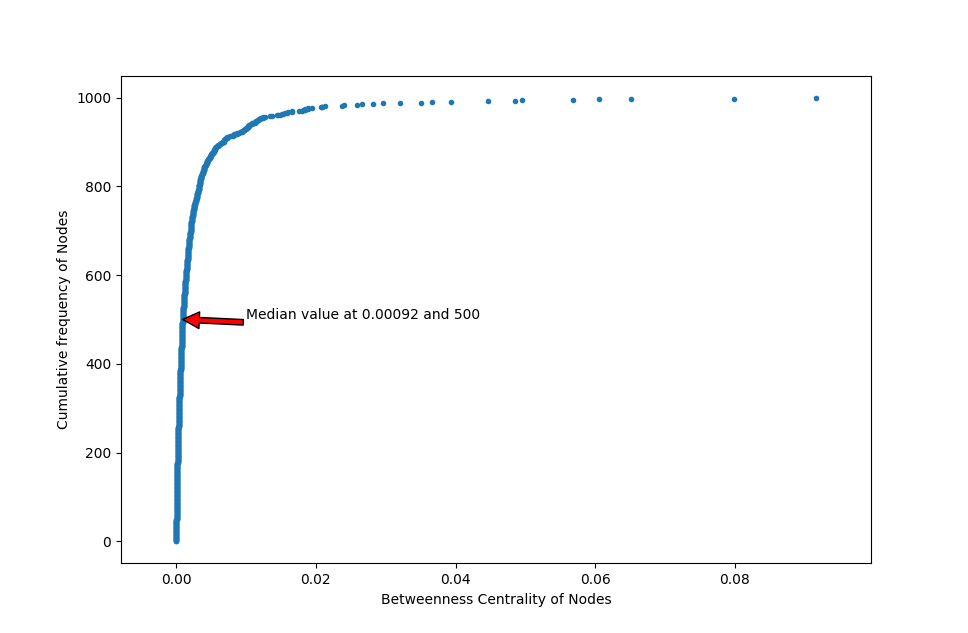
\includegraphics[width=0.45\textwidth]{image9.png}
}}
      \caption{Cumulative frequency graph for betweenness centrality (Twitter)}
      \label{figurelabel}
   \end{figure}
   
\subsubsection{Betweenness Centrality}
From the cumulative frequency distributions of the betweenness centrality values of the two networks in Figure 7 and Figure 8, it is seen that the Twitter network has a higher median value of 0.00092 whereas the Google+ network has a median of 0.00070 which is lower than this. A higher value here indicates a more cohesive network. This implies that Twitter users in these samples are more connected to each other, than Google+ users. This also means that it is easier for a user to find another user through known followers on Twitter than it is through their circles on Google+.

\subsection{Statistics Not Supporting Hypothesis}

\subsubsection{Louvain Method for Communities in large networks \cite{c8}}

\begin{table}[htb]
\caption{Number of Communities}
\begin{center}
\begin{tabular}{ | l | l | l |} 
\hline
& \textbf{Google+} & \textbf{Twitter}\\[0.5ex]
\hline
Sample 1 & 7 & 15\\
Sample 2 & 72 & 44\\
Sample 3 & 152 & 27\\[0.5ex]
\hline
\textbf{Average Value} & \textbf{77} & \textbf{28.7}\\[0.5ex]
\hline
\end{tabular}
\end{center}
\end{table}

The number of communities in these networks have been calculated using the Louvain Method (LM) \cite{c8}, which is a very efficient method for computing communities in large networks. The results however are somewhat in contradiction to what the other measures have indicated thus far. The number of communities that were observed in the samples and their averages are shown in Table V.



It can be argued that a network which contains more communities is more cohesive than a network with fewer numbers of communities. Although, a sub-graph with only 7 communities for Google+ is also observed, the average is far more than Twitter over the 3 samples taken.
However, it is worth mentioning that the Modularity values, which are a direct result of the application of LM for Twitter is significantly high than in Google+.

% \subsection{Headings, etc}

% Text heads organize the topics on a relational, hierarchical basis. For example, the paper title is the primary text head because all subsequent material relates and elaborates on this one topic. If there are two or more sub-topics, the next level head (uppercase Roman numerals) should be used and, conversely, if there are not at least two sub-topics, then no subheads should be introduced. Styles named ÒHeading 1Ó, ÒHeading 2Ó, ÒHeading 3Ó, and ÒHeading 4Ó are prescribed.

% \subsection{Figures and Tables}

% Positioning Figures and Tables: Place figures and tables at the top and bottom of columns. Avoid placing them in the middle of columns. Large figures and tables may span across both columns. Figure captions should be below the figures; table heads should appear above the tables. Insert figures and tables after they are cited in the text. Use the abbreviation ÒFig. 1Ó, even at the beginning of a sentence.

% \begin{table}[h]
% \caption{An Example of a Table}
% \label{table_example}
% \begin{center}
% \begin{tabular}{|c||c|}
% \hline
% One & Two\\
% \hline
% Three & Four\\
% \hline
% \end{tabular}
% \end{center}
% \end{table}


%   \begin{figure}[thpb]
%       \centering
%       \framebox{\parbox{3in}{We suggest that you use a text box to insert a graphic (which is ideally a 300 dpi TIFF or EPS file, with all fonts embedded) because, in an document, this method is somewhat more stable than directly inserting a picture.
% }}
%       %\includegraphics[scale=1.0]{figurefile}
%       \caption{Inductance of oscillation winding on amorphous
%       magnetic core versus DC bias magnetic field}
%       \label{figurelabel}
%   \end{figure}
   

% Figure Labels: Use 8 point Times New Roman for Figure labels. Use words rather than symbols or abbreviations when writing Figure axis labels to avoid confusing the reader. As an example, write the quantity ÒMagnetizationÓ, or ÒMagnetization, MÓ, not just ÒMÓ. If including units in the label, present them within parentheses. Do not label axes only with units. In the example, write ÒMagnetization (A/m)Ó or ÒMagnetization {A[m(1)]}Ó, not just ÒA/mÓ. Do not label axes with a ratio of quantities and units. For example, write ÒTemperature (K)Ó, not ÒTemperature/K.Ó

\section{CONCLUSION}

Twitter remains an example of a social network which has dominated the OSN ecosystem with high engagement and reciprocity values between, entrants within the OSN market would benefit from aspiring to, if not emulating the characteristics of the Twitter social network. Whereas, Google+ has tried and ultimately failed to deliver a unique and tailored user experience, which is reflected in the network statistics analysed in the Results, data set and Statistics sections of this report. Although, the number of communities within the Google+ network far outweighs those shown within Twitter, it could be argued that this formation took place during the initial period of growth that followed the release of the Google+ OSN which saw number of users increase from 19 million to 40 million as identified by Schi\"oberg et al \cite{c13}. Moreover, statistics from the analysis indicate that users from Twitter are more inclined to cluster into communities, as shown by the higher values of clustering coefficient, indicating higher user engagement and a more successful OSN overall.

Following the results of the analysis, it can be concluded that there is indeed an observable, consistent trend of the Twitter network demonstrating more robustness than the Google+ network in most of our chosen metrics and especially for the two main algorithms this paper tries to focus on - degree assortativity and the Garlaschelli and Loffredo definition of reciprocity. 

\addtolength{\textheight}{-12cm}   % This command serves to balance the column lengths
                                  % on the last page of the document manually. It shortens
                                  % the textheight of the last page by a suitable amount.
                                  % This command does not take effect until the next page
                                  % so it should come on the page before the last. Make
                                  % sure that you do not shorten the textheight too much.

%%%%%%%%%%%%%%%%%%%%%%%%%%%%%%%%%%%%%%%%%%%%%%%%%%%%%%%%%%%%%%%%%%%%%%%%%%%%%%%%



%%%%%%%%%%%%%%%%%%%%%%%%%%%%%%%%%%%%%%%%%%%%%%%%%%%%%%%%%%%%%%%%%%%%%%%%%%%%%%%%



%%%%%%%%%%%%%%%%%%%%%%%%%%%%%%%%%%%%%%%%%%%%%%%%%%%%%%%%%%%%%%%%%%%%%%%%%%%%%%%%
\section*{APPENDIX}

\subsection{Visuals Generated on Gephi}
Visuals generated on Gephi with the Fruchterman Reingold layout.
Gravity: 5.0 | Speed: 10.0 | Area: 10,000.0

\begin{figure}[!htb]
      \centering
      \framebox{\parbox{3in}{
      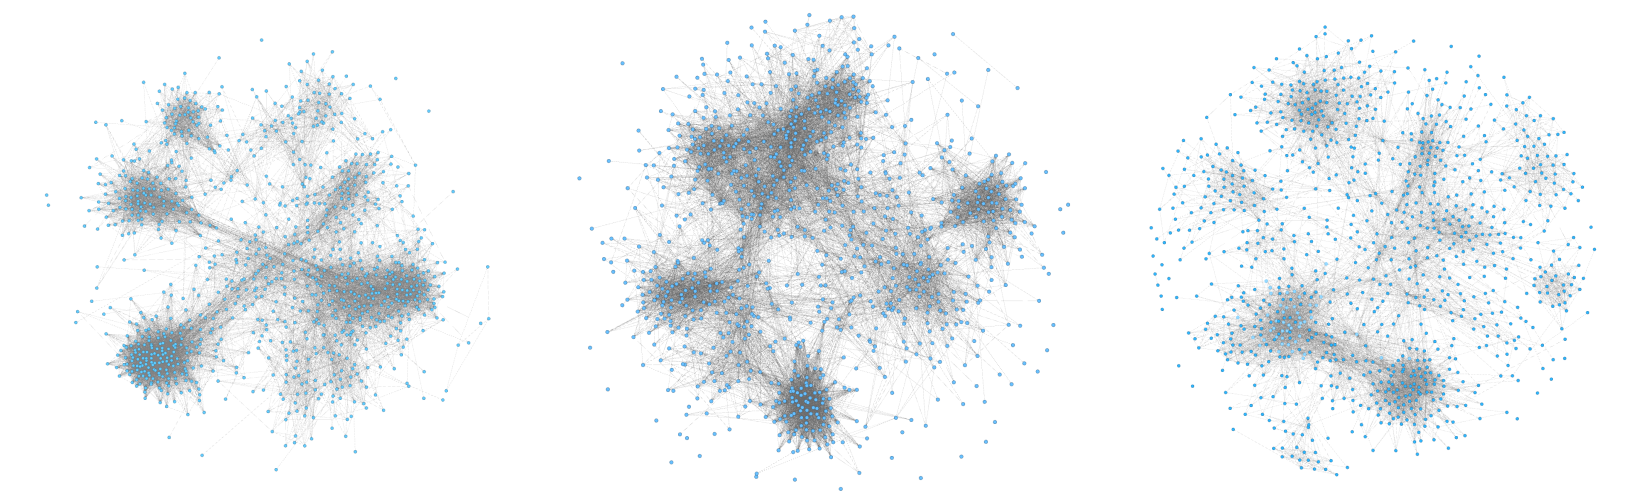
\includegraphics[width=0.40\textwidth]{images/a.png}}}
        \caption{Networks of Twitter's Samples}
\end{figure}
\pagebreak
\begin{figure}[!htb]
      \centering
      \framebox{\parbox{3in}{
      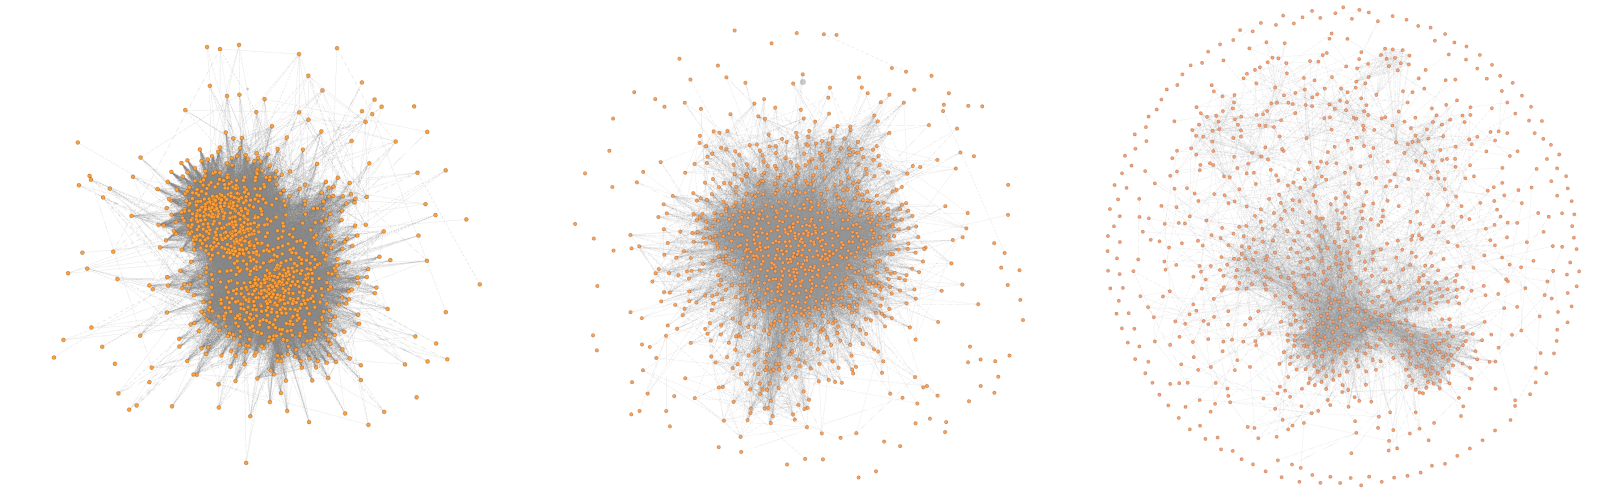
\includegraphics[width=0.40\textwidth]{images/b.png}}}
      \caption{Networks of Google+'s Samples}
      \label{figurelabel}
\end{figure}
\vspace{-2mm}
\subsection{Code Snippets}

\begin{figure}[thpb]
      \centering
      \framebox{\parbox{3in}{
      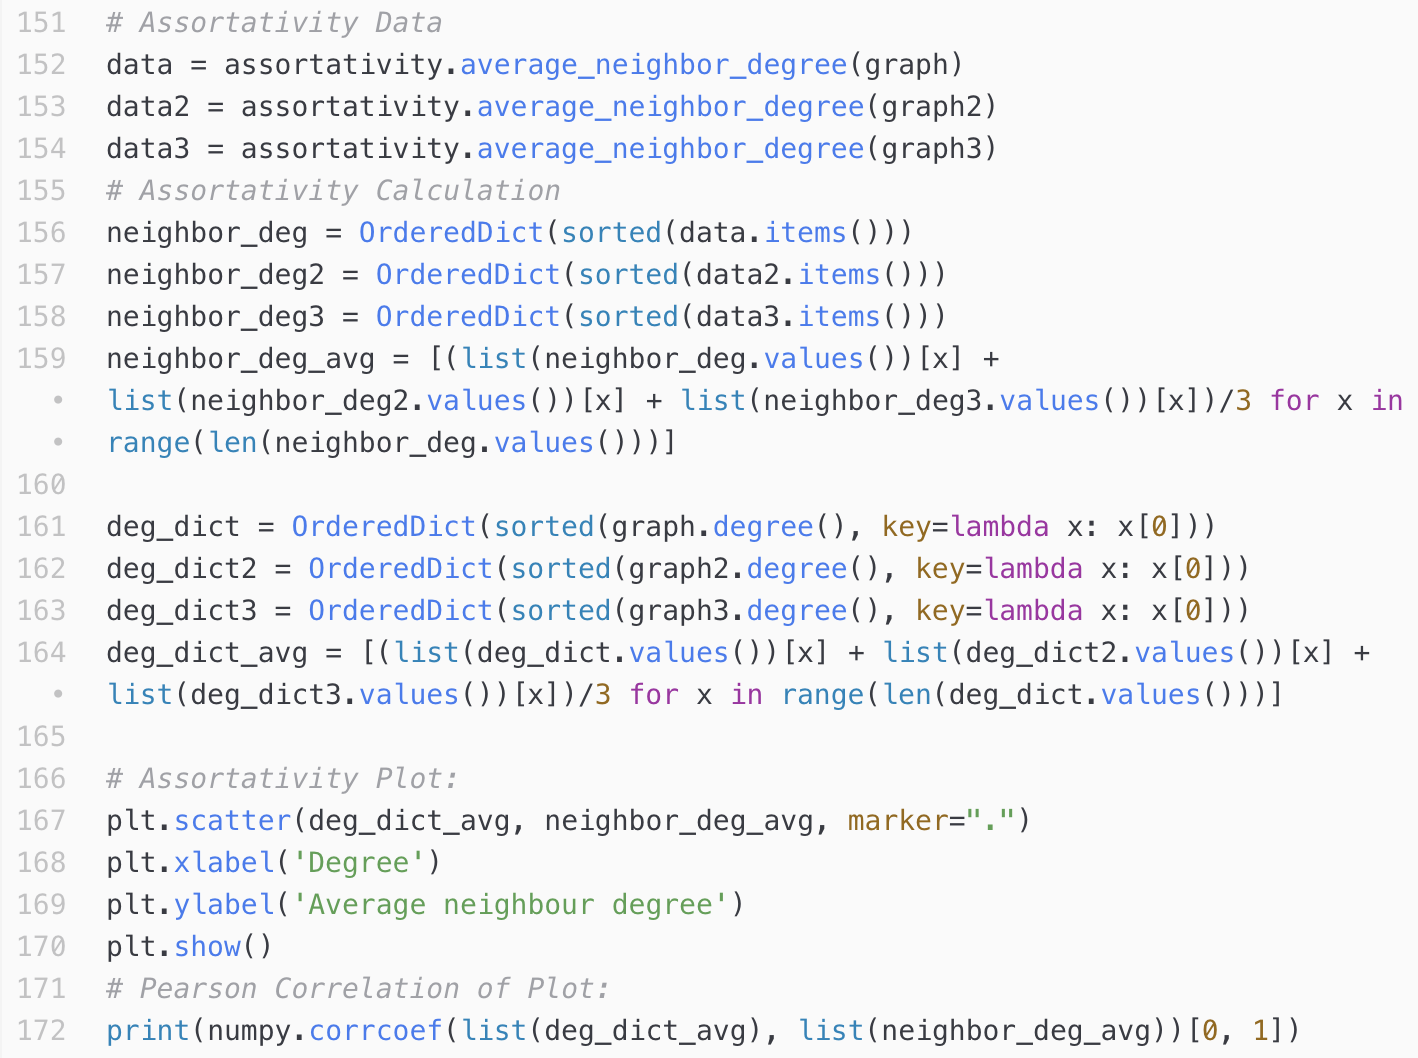
\includegraphics[width=0.43\textwidth]{images/codeSnippets/assortativityCode.png}}}
      \caption{Code snippet for degree assortativity analysis}
    \vspace{2mm}
      \framebox{\parbox{3in}{
      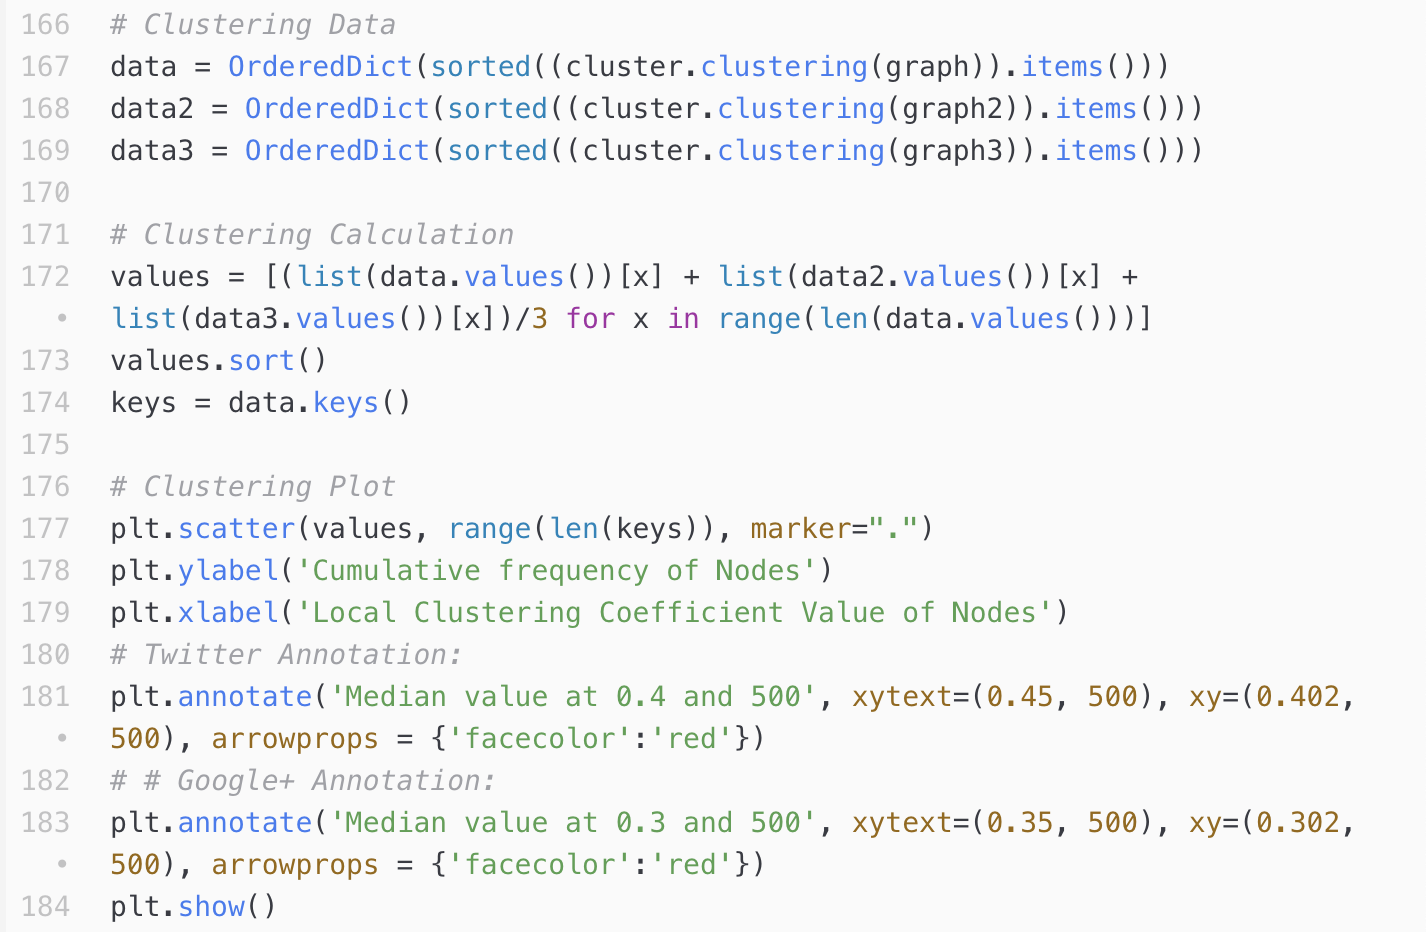
\includegraphics[width=0.43\textwidth]{images/codeSnippets/clusteringCode.png}}}
      \caption{Code snippet for local clustering coefficient analysis}
    \vspace{2mm}
      \framebox{\parbox{3in}{
      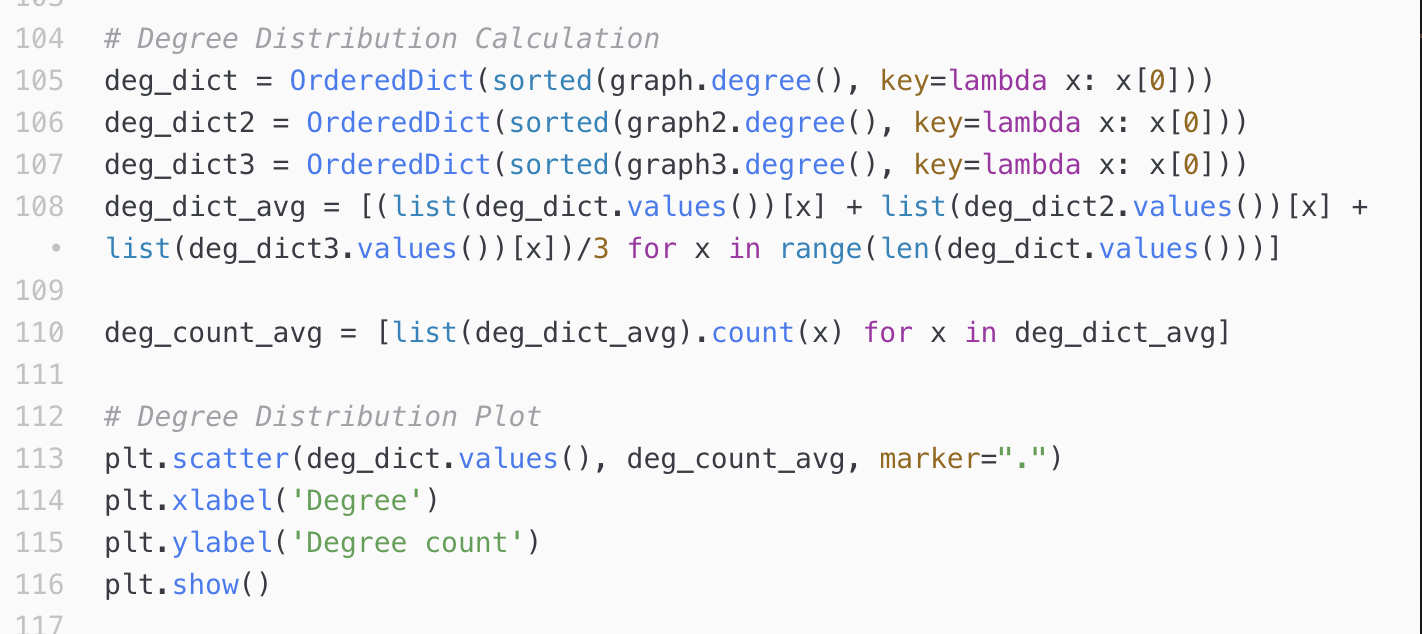
\includegraphics[width=0.43\textwidth]{images/codeSnippets/degreeCode.png}}}
      \caption{Code snippet for producing degree distribution}
      \vspace{2mm}
      \framebox{\parbox{3in}{
      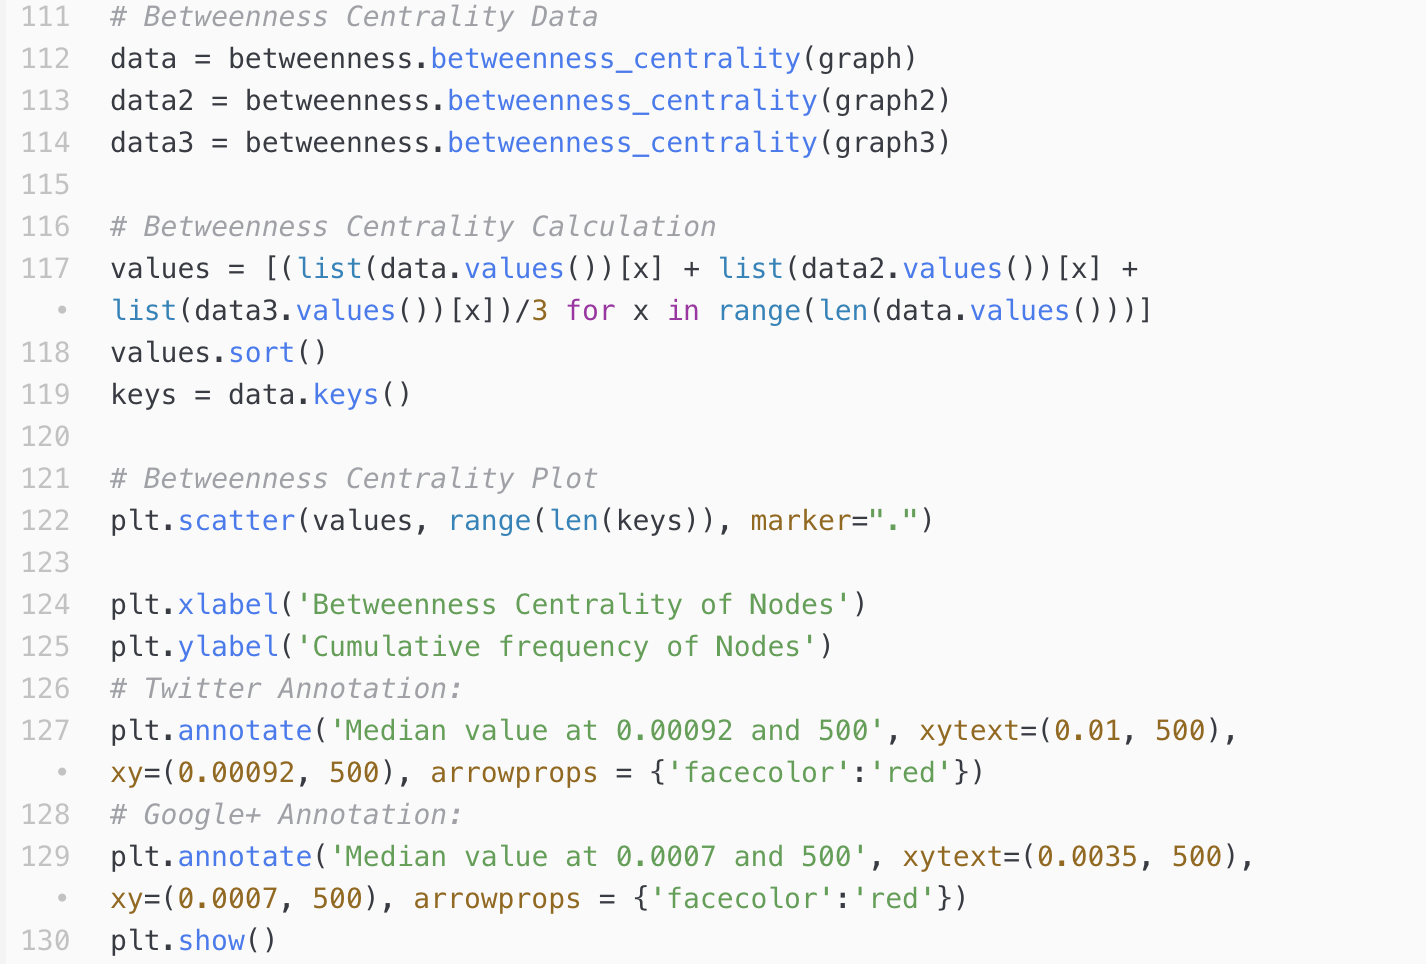
\includegraphics[width=0.43\textwidth]{images/codeSnippets/betweennessCode.png}}}
      \caption{Code snippet for betweenness centrality analysis}
\end{figure}
\clearpage
%%%%%%%%%%%%%%%%%%%%%%%%%%%%%%%%%%%%%%%%%%%%%%%%%%%%%%%%%%%%%%%%%%%%%%%%%%%%%%%%

% References

\begin{thebibliography}{99}

\bibitem{c1}B. Smith, "Project Strobe: Protecting your data, improving our third-party APIs, and sunsetting consumer Google+", Google, 2018. [Online]. Available: https://www.blog.google/technology/safety-security/project-strobe/. [Accessed: 24- Mar- 2019]
\bibitem{c2}S. Gaudin, "Astronauts, Obama to host Google+ hangouts", Computerworld, 2013. [Online]. Available: https://www.computerworld.com/article/2494873/astronauts--obama-to-host-google--hangouts.html. [Accessed: 21- Mar- 2019]
\bibitem{c3}"We hear you: Better commenting coming to YouTube", Official YouTube Blog, 2013. [Online]. Available: https://youtube.googleblog.com/2013/09/youtube-new-comments.html. [Accessed: 21- Mar- 2019]
\bibitem{c4}S. Rich, "How Google Plus Helps Your SEO and Online Marketing", Digital Doughtnut, 2017. [Online]. Available: https://www.digitaldoughnut.com/articles/2017/january/how-google-plus-helps-your-seo-and-online-marketin. [Accessed: 21- Mar- 2019]
\bibitem{c5}S. Si, "How does Google Plus Affect SEO?", Basic and Advanced SEO Tutorials and News - SEO Hacker Blog, 2019. [Online]. Available: https://seo-hacker.com/google-affect-seo/. [Accessed: 21- Mar- 2019]
\bibitem{c6}D. Choate, "Google Plus in 2018: Who's Using It and Why | Raka", Raka, 2016. [Online]. Available: https://www.rakacreative.com/blog/social-media-marketing/what-is-google-plus-2018/. [Accessed: 21- Mar- 2019]
\bibitem{c7}R. Hof, "Google Still Struggles To Explain Why Normal People Should Care About Google+", Forbes.com, 2013. [Online]. Available: https://www.forbes.com/sites/roberthof/2013/05/16/google-still-struggles-to-explain-why-real-people-should-care-about-google/. [Accessed: 21- Mar- 2019]
\bibitem{c8}V.D.Blondel, JL.Guillaume, R.Lambiotte, E.Lefebvre, "Fast unfolding of communities in large networks. Journal of Statistical Mechanics: Theory and Experiment", Vol.2008. 10008. 2008. [Online] Available: https://arxiv.org/pdf/0803.0476.pdf [Accessed: 10th March 2019]
\bibitem{c9}D. Garlaschelli,  M. I.Loffredo,  "Patterns of Link Reciprocity in Directed Networks. Physical Review Letters", Vol.93(26).268701. 2004. [Online]. Available:  https://arxiv.org/pdf/cond-mat/0404521.pdf [Accessed: 10th March 2019]
\bibitem{c10}Leskovec, Jure and Sosi. SNAP: A General-Purpose Network Analysis and Graph-Mining Library, Social Circles: Twitter. ACM Transactions on Intelligent Systems and Technology (TIST). Vol. 8(1). 1. Stanford, California. Stanford University. 2016. [Online]. Available: https://snap.stanford.edu/data/ego-Twitter.html  [Accessed: 10th Feb 2019]
\bibitem{c11}Leskovec, Jure and Sosi. SNAP: A General-Purpose Network Analysis and Graph-Mining Library, Social Circles: Google+. ACM Transactions on Intelligent Systems and Technology (TIST). Vol. 8(1). 1. Stanford, California. Stanford University. 2016. [Online]. Available: https://snap.stanford.edu/data/ego-Gplus.html  [Accessed: 10th Feb 2019]
\bibitem{c12}M.E.J. Newman, "Mixing patterns in networks", Physical Review E. Vol.67(2). 026126. 2003. [Online]. Available: https://arxiv.org/pdf/cond-mat/0209450.pdf  [Accessed: 10 Feb 2019]
\bibitem{c13}D. Schi\"oberg, F. Schneider, H. Schi\"oberg, S.Schmid, S. Uhlig, A.Feldmann, "Tracing the birth of an OSN: social graph and profile analysis in Google+". 265-274. 2012. [Online]. Available: https://www.net.t-labs.tu-berlin.de/~stefan/websci12.pdf   [Accessed: 10 Feb 2019]
\bibitem{c14}J.D.Watts, S.H.Strogatz, "Collective dynamics of ‘small-world’ networks", Nature. Vol.393. 440-442.1998. [Online]. Available: https://www.nature.com/articles/30918.pdf  [Accessed: 20 Feb 2019]
\bibitem{c15}B.Paolo, R. Marco, V.Sebastiano, Singapore.Springer-Verlag, "Robustness of Social Networks: Comparative Results Based on Distance Distributions", 2011. pp.13-17. [Online]. Available: https://arxiv.org/pdf/1110.4474.pdf [Accessed: 20 March 2019]

\end{thebibliography}
\end{document}
